\chapter{Attack Vectors}


\section{Exhaustive Search Attack}
    The Exhaustive search attack, or brute-force attack, is to try every key possible until we retrieve the plaintext message. Although very crude and somewhat inefficient, some ciphers are unfortunately weak against it: the DES is one of them.
    
\paragraph{Definition :}
Given $(m_i,c_i)$ in $\llbracket 1,N \rrbracket$(with N a small integer), find key k.

\paragraph{DES Challenge (by RSA)\\}
The aim of the DES Challenge is to find the secret key given three messages and their encryption. It was organized by the RSA company, to demonstrate the vulnerability of DES (the good ol' naming and shaming technique ).

\begin{description}
\item[1997 : ] 3 months using Internet-distributed computation ("cloud" computing)
\item[1998 : ] 3 days using EFF\footnote{Electronic Frontier Foundation : a NGO focusing on net freedom}'s deep crack machine.
\item[1999 : ] 22 hours
\item[2006 : ] 7 days using 10k\$'s FPGAs.
\end{description}

\paragraph{Prevention}
You only way to prevent a cipher from ESA is to augment the key size until no existing computation power can break the cipher in a reasonable time (like centuries).

\section{Cryptographic attacks}
The cryptographic attacks are the generic attack types used when talking about theoretical security (like semantic security).

\paragraph{Known Plaintext  \\} The attacker has in his possession a plaintext message and its corresponding encryption.

\paragraph{Cyphertext Only  \\} The attacker does not know the plaintext message and has to find out (see Cesar cipher's breaking technique).

\paragraph{Chosen Plaintext/Cyphertext \\} 
The attacker can respectively encrypt/decrypt any plaintext/cyphertext message and study the result. It is the most common paradigm when studying public key cryptography (the attacker know the public key and can encrypt any message of his will).

\paragraph{Adaptative Plaintext/Cyphertext \\} 
The attacker can iterate the encryption/decryption based on the previous result (used for linear and differential attacks).

\section{Side-channel attacks}
Side-channel attacks are "real-world" attacks, i.e. they don't rely on theoretical cryptographic knowledge but rather the implementation of ciphers. \footnote{ They are considered "inelegant", but the result is what matters, is it not ?}

\paragraph{Attack on the implementation \\}
Some perfectly secure ciphers can be compromised if they are implemented in the wrong way : buffer overflows on user input, stack overflows, information leaking, insufficient entropy, ...   

\paragraph{Hardware Attacks \\}
Another way to look at implementation is to consider the hardware : the analysis of the time and power required to encode/decode messages (using oscilloscopes and multimeter) can reveal important informations about the cipher used.

\paragraph{Fault Attacks \\}
This attack is a follow up of the previous ones : by using laser to provoke run-time segfault (by twiddling the RAM bits), the attacker's aim is to create computing errors which can reveal informations about the key.

\section{Meet in the middle attacks}

\paragraph{Definition\\}
The MITM attacks is a generic cryptoanalysis used originally to break n-rounds block ciphers. Given the ability to encrypt and decrypt any data, the attacker will try to find the encryption of a certain plaintext which match the decryption of another certain cyphertext. In others words, the encryption and decryption algorithm does each one half of the work and "meet".

\begin{mydef}[Meet in the middle Attack :]
b \newline
\begin{minipage}[t]{0.8\textwidth}
	Given (E,D) encryption/decryption system, \\
    Find (m,c) such that : E(m) == D(c).
\end{minipage}
\end{mydef}

\paragraph{Example}

A famous example which validate the theory of "more rounds equal better security" is the double-DES : once demonstrated that DES is insecure, they tried to update the standard without changing everything by simply cascading a DES into another one, using two separate keys. However, 2-DES is badly vulnerable from MITM attacks.

\begin{mydef}[Challenge :]
b \newline
\begin{minipage}[t]{0.9\textwidth}
	Given (m,c), find $k = (k_1,k_2)$ such that $E(k_1,E(k_2,m)) == c$
\end{minipage}
\end{mydef}

Since $k_1$ and $k_2$ are independent keys, we have : $E(k_2,m) = x = D(k_1,m) $ . Breaking a $2-DES$ cipher is close to break DES, just twice longer. That's why $2-DES$ was never used and standard chosen is $3-DES$.

\section{Linear and Differential Attacks}

\subsection{Linear Attacks}
\subsection{Differential Attacks}


\section{Quantum attacks}

Quantum attacks are based on quantum computing. Unlike classical computers, quantum computers take advantage of quantum state superposition and entanglement to speed up solving time of equations, especially when combinatory calculus are present.

\paragraph{ Generic Search Problem}

\begin{mydef}
\begin{minipage}[t]{0.8\textwidth}
    Let $f : X \rightarrow {0,1}$ a generic oracle, \\
  	Generic Search Problem : find $x \in X$ such as $ f(x) == true $.
\end{minipage}
\end{mydef}

On classical computer, the best generic solver is linear ( $O(|X|)$ ) whereas on a quantum computer, it's root-squared ( $O(|X|^{\frac{1}{2}})$).


\paragraph{ Consequences } 
The practical consequence of quantum computing over cryptography is to halve the key space : a way to prevent ciphers from quantum attacks is to double the key space ( a 1024-key RSA cipher is as strong against quantum computers as a 512-key RSA cipher against classical computers).


\section{Collision attacks}

When talking about collision resistance, it is important to speak about the Birthday Paradox which stipulates that there are way more random collisions than you would guess.

\subsection{Generic Birthday attacks}

The Birthday Paradox rest upon the following question : given a random group of people, what's the odds of having at least two persons with the same birthday ? The question is equivalent of estimating the probability of a collision from the output of a bounded random number generator.\\

Intuitively, we would think that the odds grow linearly with the group's size whereas, in reality, the odds grow way faster : when the group has 23 person, there is a 50\% chance of a collision ! The paradox lies here : you only need of tenth of sample from the random pool to have a fairly high chance of collision, which is not intuitive (we would rather think of needing half of the pool - more or less 180 persons -  to have a 50\% chance).

\begin{figure}[ht!]
    \centering
   	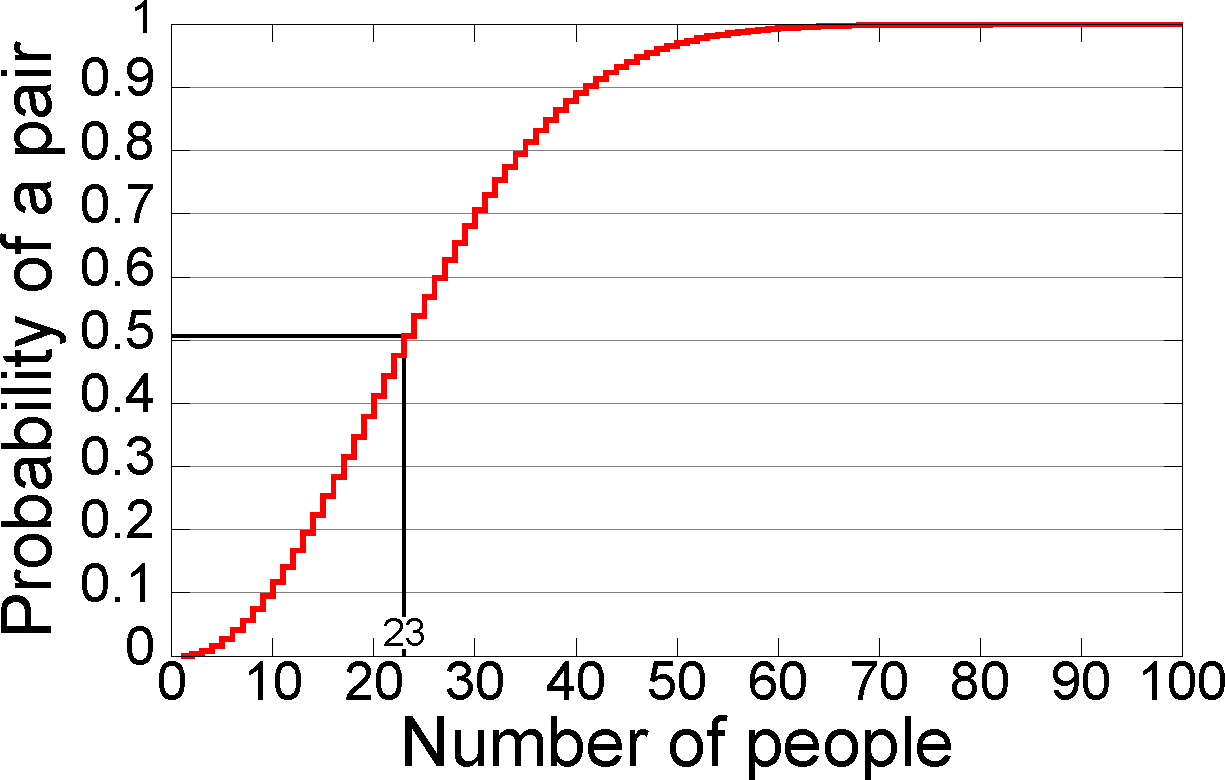
\includegraphics[width=\textwidth]{images/Birthday_Paradox.pdf}
	\caption{Probability of a match, according to the group's size \\ source : Wikipedia}
	\label{fig:BirthdayParadox}
\end{figure}

\begin{mytheorem}[Birthday Paradox]
Let $r_1,r_2,...r_n in {1,...B}$ n independent integers chosen uniformly, \\
Then, when $n = 1.2\times B^{\frac{1}{2}}$, $Pr[collision] \geq \frac{1}{2} $
\end{mytheorem}

The mathematical proof of this theorem is fairly simple : let compute the probability $Q(n,B)$ of not having a collision given n persons and B possible birthdays. Q can be seen as multiples draws without duplicates : \\
\begin{align}
    Q(n,B) =& 1 \times \frac{B-1}{B} \times ... \times \frac{B-n}{B} \\
           =& \frac{B!}{(B-n)!*B^n} \\
\end{align}  

$P(n,B)$, the probability of having a birthday collision given n persons and B possible birth dates, is $Q(n,b)$ complement. \\
Using Taylor series expansion we can rewrite $\frac{B-k}{B}$ as $e^{\frac{-k}{B}}$. 

\begin{align}
    Q(n,B) =& \prod_{k = 0}^n e^{\frac{-k}{B}}      \\
           =& e^{\sum_{k = 0}^n \frac{k}{B}}        \\
           =& e^{ \frac{-(\frac{*n(n-1)}{2})}{B} }  \\
    P(n,B) \simeq& 1 - e^{ \frac{-n^2}{2*B} }       
\end{align}  


Using the previous relation, we can easily compute $P(n,B) \geq 0.5$ and find the result presented in the theorem.\\

The attackers take advantage of the fact that a fairly low number of random guess have a reasonable chance for one of them of being correct. For example, there was a DNS spoofing method using it : \\

\begin{figure}[ht!]
    \centering
       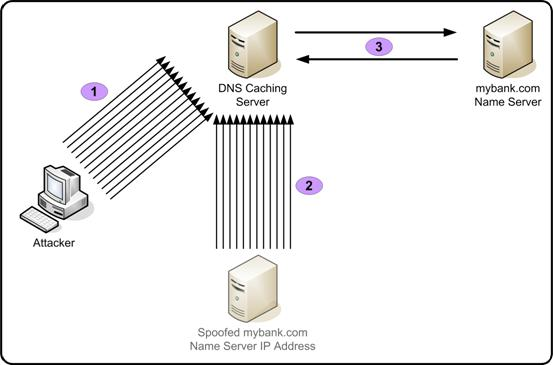
\includegraphics[width=\textwidth]{images/dns_spoofing_birthday.jpg}
	\caption{DNS Spoofing using multiple queries and Birthday Paradox \\ source : http://www.technicalinfo.net}
	\label{fig:DNSSpoofingBirthday}
\end{figure}

The attacker's aim is to trick the DNS cache server into thinking that the IP of www.mybank.com is the spoofed server's one, not the real one. This attack is used for phishing : as soon as the DNS cache server is compromised, users connecting to www.mybank.com will send their credentials to the attackers. \\
In order to do so, the attacker will send multiple queries : each DNS resolution is accompanied with a transaction ID which identify the query. The attacker's goal is to send resolution answers from this server with the correct transaction ID. The spoofed server send multiple resolution answers with random transaction ID. Since a DNS transaction ID is coded on 2 bytes, the pool of ID is no larger than 65535 : the birthday theorem stipulate that, with $n = 1.2 * \frac{\sqrt{65535}}{2}  = 153$  \footnote{ $n$ resolution queries$ + n$ answers $= 2*n$ total queries where looking for collision }queries, the attack has a 50\% chance of success\footnote{with 400 queries, the probability is over 99\%}. To further improve the probability of success, the attacker can also cripple the other server (the real one) with DDOS or bad routed packets in order to prevent him from sending a correct DNS resolution answer.

\section{Social Attacks}

Attacks target the weakest link of a system : sometimes it is the human nature the weakest link. This finding led to the famous "social engineering" attacks and the less known (but way more dangerous) rubberhose attacks.

\paragraph{Social Engineering}

Social Engineering describe a motley crew of methods designed to "punching a hole" into a system from the inside, without informing the insider of what he has done. \\
The most famous example is to leave some booby-trapped pendrives (and even more creative methods 
\footnote{ A mouse device with modified firmware was sent as a gift to tech-based company employees for a security test : \url{ http://www.theregister.co.uk/2011/06/27/mission_impossible_mouse_attack/}.  }
) on the company site and hope for one employee to plug it in his workstation . Once it is plugged, the rigged pendrive which usually contains a Trojan, execute its script in order to obtain a privilege escalation from within the system and connect to the attacker then.\\\\
A new type of Social Engineering has arisen with the emergence of social networks (Facebook, LinkedIn, ...) : in this type of attacks, the goal is to obtain a remote account of a target using infos about disseminated around the Web (email addresses, universities he has been, birthday, birth place, ...) and use it to gain access to his email account (using password reset and secret questions). Once the email account has been compromised, it can be used to launch phishing attacks on the real target and retrieve important secrets.


\paragraph{Rubberhose Cryptoanalysis}

The rubberhose attack describe the use of force (legal, hierarchical or physical) and/or torture on a physical person in order to extract information about the system (keys, ciphers used, ...). It is difficult to prevent those attacks since they are outside the scope of cryptanalysis (most of them belong to sociology/politics). The only way to mitigate against those attacks would be agent partial-blindness or plausible deniability.

\begin{figure}[hb!]
    \centering
       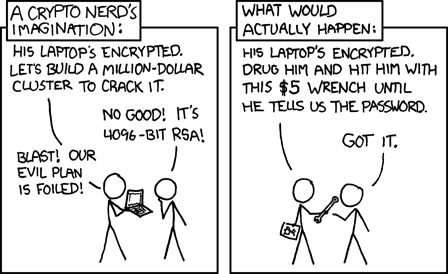
\includegraphics[width=0.7\textwidth]{images/rubberhose.png}
	\caption{Real-world 0-day exploit. \\ source : XKCD}
	\label{fig:RC4}
\end{figure}
